\documentclass[12pt, twoside]{article}
\usepackage[francais]{babel}
\usepackage[T1]{fontenc}
\usepackage[latin1]{inputenc}
\usepackage[left=1cm, right=1cm, top=6mm, bottom=6mm]{geometry}
\usepackage{float}
\usepackage{graphicx}
\usepackage{array}
\usepackage{multirow}
\usepackage{amsmath,amssymb,mathrsfs}
\pagestyle{empty}

\begin{document} 
\begin{center}
{\fbox{$2^{de}5$ \qquad \qquad \textbf{\large{Devoir surveill� 2}}
\qquad \qquad 24/10/2008}}
\end{center}

\textbf{NOM Pr�nom:} \ldots \ldots \ldots \ldots \ldots \ldots
\bigskip

\textbf{Exercice 1:} \textit{5 points} 
\begin{enumerate}
  \item Compl�ter le tableau suivant (en couleur visible pour la droite
  gradu�e):

  \begin{tabular}{|m{55mm}|c|m{35mm}|m{35mm}|m{20mm}|}
\hline
Texte & Intervalles & Repr�sentation sur une droite gradu�e & Ensemble
des r�els $x$ v�rifiant: & L'ensemble est-il born�? (oui ou non)\\
\hline
l'ensemble des r�els compris entre $-13$ inclu et $\sqrt{2}$ exclu & & & &
\\[7mm]
\hline
& $]-\infty;\sqrt{6}[$& & & \\[7mm]
\hline
& & 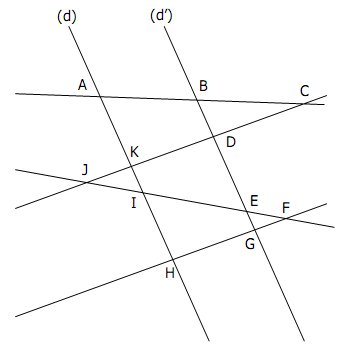
\includegraphics[width=3cm]{images/ex1.jpg}
 & & \\[7mm]
\hline
 & & & $x \geqslant 1$ & \\[7mm]
\hline

\end{tabular}


\medskip



\item Soit $I=]-7;\ 1,2]$.\\
Est ce que $-7 \in I$? \dots \dots \dots \dots \\
Est ce que $1,2 \in I$? \ldots \ldots \ldots \ldots \\
Donner un rationnel non d�cimal de $I$: \ldots \ldots \ldots \ldots \\
\end{enumerate}

\bigskip
\bigskip

\begin{center}
{\fbox{$2^{de}5$ \qquad \qquad \textbf{\large{Devoir surveill� 2}}
\qquad \qquad 24/10/2008}}
\end{center}

\textbf{NOM Pr�nom:} \ldots \ldots \ldots \ldots \ldots \ldots

\bigskip


\textbf{Exercice 1:} \textit{5 points} 
\begin{enumerate}
  \item Compl�ter le tableau suivant (en couleur visible pour la droite
  gradu�e):

  \begin{tabular}{|m{55mm}|c|m{35mm}|m{35mm}|m{20mm}|}
\hline
Texte & Intervalles & Repr�sentation sur une droite gradu�e & Ensemble
des r�els $x$ v�rifiant: & L'ensemble est-il born�? (oui ou non)\\
\hline
l'ensemble des r�els compris entre $-13$ inclu et $\sqrt{2}$ exclu & & & &
\\[7mm]
\hline
& $]-\infty;\sqrt{6}[$& & & \\[7mm]
\hline
& & 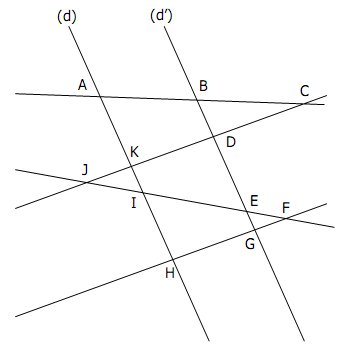
\includegraphics[width=3cm]{images/ex1.jpg}
 & & \\[7mm]
\hline
 & & & $x \geqslant 1$ & \\[7mm]
\hline

\end{tabular}


\medskip



\item Soit $I=]-7;\ 1,2]$.\\
Est ce que $-7 \in I$? \dots \dots \dots \dots \\
Est ce que $1,2 \in I$? \ldots \ldots \ldots \ldots \\
Donner un rationnel non d�cimal de $I$: \ldots \ldots \ldots \ldots \\
\end{enumerate}
\end{document}
